%!TEX root = ../dissertation.tex
\chapter{OpenCog System} \label{cha:opencog_system}

The OpenCog design aims to capture the spirit of the architecture and dynamics of the brain without imitating the details (which are largely unknown) via:
\begin{itemize}
	\item Integrating together a carefully selected combination of cognitive algorithms acting on different kinds of knowledge.
	\item A scalable, robust and flexible C++ software architecture.
	\item A manner specifically designed:
	\begin{itemize}	
	\item To cooperate together with “cognitive synergy” for the scope of tasks characteristic of human intelligence. 
	\item To give rise to the emergence of an effectively functioning knowledge network in the AI system’s mind, as it interacts with the world, including a self-updating hierarchical/heterarchical ontology and models of itself and others.
	\end{itemize}
\end{itemize}
Following section, Section \ref{sec:cognitive_synergy}, elaborates on the new concepts introduced in these points.


\section{Cognitive Synergy}\label{sec:cognitive_synergy}  %% slide 4 tua presentazione, magari aggiungi le parte in basso

OpenCog is a diverse assemblage of cognitive algorithms, each embodying its own innovations. The power of the overall architecture is its careful adherence to the principle of Cognitive Synergy. \\
The human brain consists of a host of subsystems that perform particular tasks, both specialized and general in nature, connected together in a manner enabling them to synergetically assist, rather than work against each other. \\
The essential principles of Cognitive Synergy Theory (CST) can be summarized in the following points, further explored in \cite{inproceedings_cognitive_synergy}:

\begin{enumerate}
	\item Intelligence can be understood as the ability to achieve complex goals in a certain set of environments. 
	\item An intelligent system requires a \enquote{multi-memory} architecture, meaning the possession of a number of specialized yet interconnected knowledge types.
	\item \enquote{Cognitive processes}: a system must possess knowledge creation mechanisms corresponding to each of these memory types.
	\item Each cognitive process must have the ability to recognize when it lacks information and thus, draw it from knowledge creation mechanisms related to other types of knowledge.
	\item The Cognitive Synergy is, therefore, represented by the interaction between the knowledge creation mechanisms, which perform much more effectively in combination than non-interactive mode. 
	\item The activity of the different cognitive processes involved in an intelligent system can be modeled in terms of the schematic implication \enquote{Context \& Procedure $\rightarrow$ Goal}.
\end{enumerate}

These points are implicit in the systems theory of mind given in \cite{goertzel2006the}, where more thorough characterizations of these ideas can be found.\\
Interactions as mentioned in Points 4 and 5 are the conceptual core of CST. \\
Most AI algorithms suffer from combinatorial explosions. In a “general intelligence” context, there is a lack of intrinsic constraint; consequently, the algorithms are unable to filter through all the possibilities (as opposed to a ANI problem like chessplaying, where the context is huge but constrained and hence restricts the scope of possible combinations that needs to be considered). \\
To decrease the severity of combinatorial explosions, one can use an AGI architecture based on CST, in which the different learning mechanisms dealing with a certain sort of knowledge, are designed to synergize with ones dealing with other sorts of knowledge. \\
It is necessary that each learning mechanism recognizes when it is \enquote{blocked} and then, it can ask for help to the other complementary cognitive mechanisms. \\
The Figure \ref{fig:cognitive_processes} is proposed to give a general visual idea of these concepts. It shows an overview of the most important cognitive dynamics considered in Cognitive Synergy Theory and describes the behavior of a system as it pursues a set of goals, which are then refined by inference (through a logic engine or as an emergent process resulting from the dynamics of an Neural Network system), aided by other processes. \\


\begin{figure}
\centering
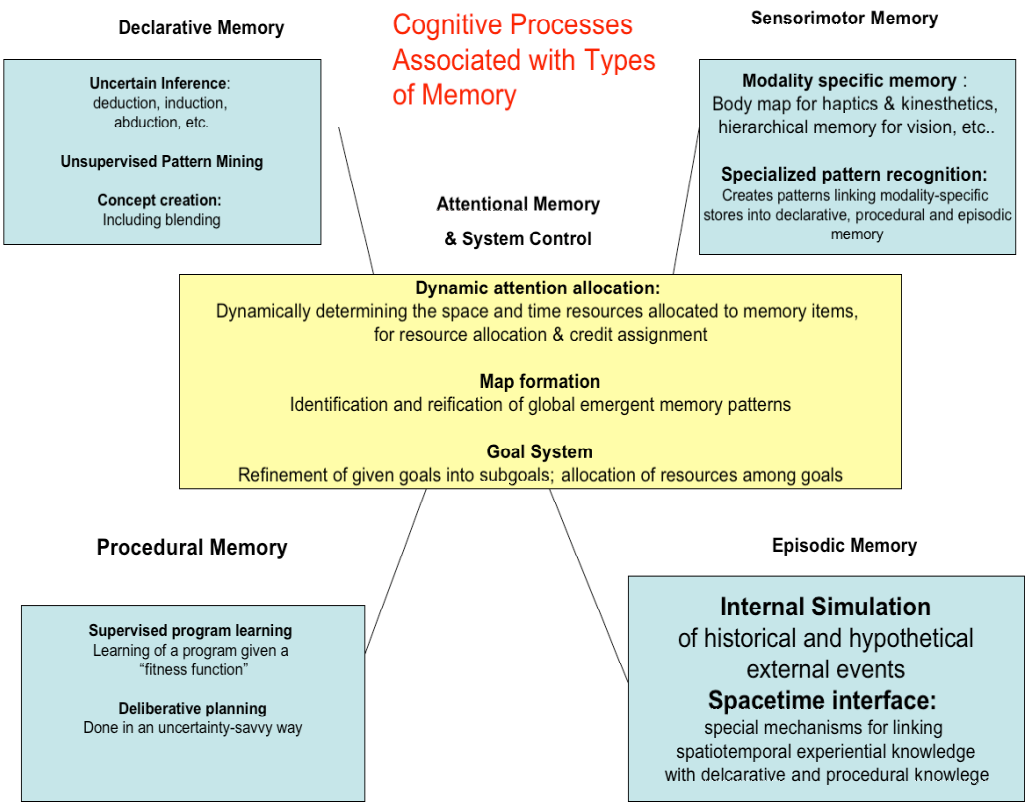
\includegraphics[width=0.7
\textwidth]{figures/Magistrale/04 - cognitive_processes_and_memory}
\caption[Cognitive Processes.]{A high-level overview of the main types of cognitive process considered in Cognitive Synergy Theory, categorized according to the type of knowledge with which each process deals.
\label{fig:cognitive_processes}}
\end{figure} 

The detailed argument explaining how the cognitive algorithm selection and integration methods, chosen by the OpenCog team, will have the desired effect, is sketched on the OpenCog wiki site\footnote{\url{https://wiki.opencog.org/w/Background_Publications}} and various previously-published conference papers. It has been presented more thoroughly in the 2014 books Engineering General Intelligence vol. 1 and 2 \cite{DBLP:series/atlantis/GoertzelPG14, DBLP:series/atlantis/GoertzelPG14a}.

\section{OpenCog Architecture}\label{sec:opencog_architecture}

There are several components that make up the basic architecture of OpenCog. In the following sections, they will be described, more or less independently, and then concatenated and contextualized into the problem considered in this project. \\
Currently, the OpenCog project is under strong development and some of the concepts presented here may be obsolete, improved or evolved, or being redesigned. However, much of the basic infrastructure and theory remains unchanged.  

\subsection{Atomspace}\label{sec:atomspace}

The AtomSpace is a platform for building Artificial General Intelligence (AGI) systems. It provides the central knowledge representation component for OpenCog. As such, it is a fairly mature component, on which a lot of other systems are built, and which depend on it for stable, correct operation in a day-to-day production environment. \\
It is a mashup of a large variety of concepts from mathematical logic, theorem proving, graph theory, database theory, type theory, model theory and knowledge representation. \\
More specifically, the OpenCog AtomSpace is an in-RAM knowledge representation database, an associated query engine and graph-re-writing system, and a rule-driven inferencing engine that can apply and manipulate sequences of rules to perform reasoning. \\
The best way to capture all of this, is a kind of in-RAM Generalized Hypergraph (Metagraph) Database. \\
On top of this, the Atomspace provides a variety of advanced features not available anywhere else. It is currently used to store natural language grammars, dictionaries and parsers, to store biochemical and biomedical data, robot control algorithms, machine learning algorithms, audio/video processing pipelines and deep learning neural networks.\\

\subsubsection{Metagraph: a Generalized Hypergraph}\label{sec:gen_hypergraph}

Formally, a graph is:
\begin{itemize}
	\item A set of vertexes $V=\left\{v_{1}, v_{2}, \cdots, v_{M}\right\}$
	\item A set of edges $E=\left\{e_{1}, e_{2}, \cdots, e_{N}\right\}$ where each edge $e_{k}$ is an ordered pair of vertexes drawn from the set $V$.
\end{itemize}
Since edges are ordered pairs, it is conventional to denote them with arrows. In practice, one wishes to associate a label to each vertex, and also some additional attribute data (e.g. weight); likewise for the edges. \\

A hypergraph is very similar to a graph, except for the edges. 
\enquote{Hyperedges} are defined as edges that can contain more than two vertices. That is, the hyperedge, rather than being an ordered pair of vertices, is an ordered list of vertices. \\
Formally, a hypergraph is:
\begin{itemize}
	\item A set of vertexes $V=\left\{v_{1}, v_{2}, \cdots, v_{M}\right\}$
	\item A set of hyperedges $E=\left\{e_{1}, e_{2}, \cdots, e_{N}\right\}$ where each hyperedge $e_{k}$ is an ordered list of vertexes drawn from the set $V$. This list may be empty, or have one, or two, or more members.
\end{itemize}

A good representation of a hypergraph is the one proposed in Figure \ref{fig:atomspace_table}. 
It was a straight-forward extension of the edge table, to which a new column was added for each position and then, those columns were mashed together into one set.  

\begin{figure}
\centering
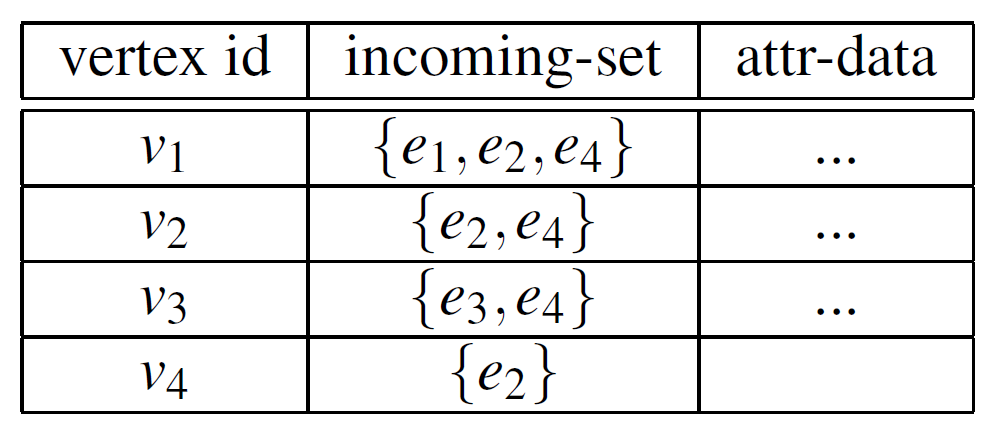
\includegraphics[width=0.7
\textwidth]{figures/Magistrale/atomspace_table}
\caption[]{Hypergraph edge table
\label{fig:atomspace_table}}
\end{figure}

The vertex table looks like the edge table, but the vertex-list is an ordered list, while the incoming-set (the edge-set) really is a set. This is because a hypergraph is “almost” a bipartite graph, having the form of Figure \ref{fig:hypergraph_graph}, with the set E on the left being the set of hyperedges. \\

\begin{figure}
\centering
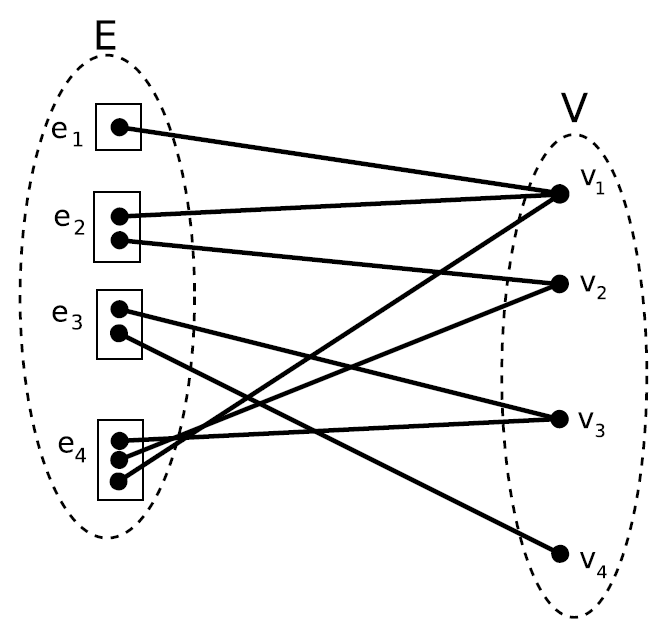
\includegraphics[width=0.6
\textwidth]{figures/Magistrale/hypergraph_graph}
\caption[]{The $E$ and $V$ ellipses are the hyperedge and vertex tables. The boxes mean that the hyperedges are ordered lists.
\label{fig:hypergraph_graph}}
\end{figure}

Before define a Metagraph, a change of terminology is useful: the basic objects are now called \enquote{Nodes} and \enquote{Links} instead of \enquote{vertexes} and \enquote{edges}. \\
Thus, a Metagraph is:
\begin{itemize}
	\item A set of nodes $V=\left\{v_{1}, v_{2}, \cdots, v_{M}\right\}$
	\item A set of links $E=\left\{e_{1}, e_{2}, \cdots, e_{N}\right\}$ where each hyperedge $e_{k}$ is an ordered list of nodes, or other links, or a mixture. They are arranged to be acyclic (to form a directed acyclic graph).
\end{itemize}

The metagraph is a generalization of a hypergraph, in the sense that now a hyperedge (link) may contain either another vertex (node) or another link. Visually, it has the shape of a Directed Acyclic Graph (DAG), such as the one shown in Figure \ref{fig:metagraph_graph}.

\begin{figure}
\centering
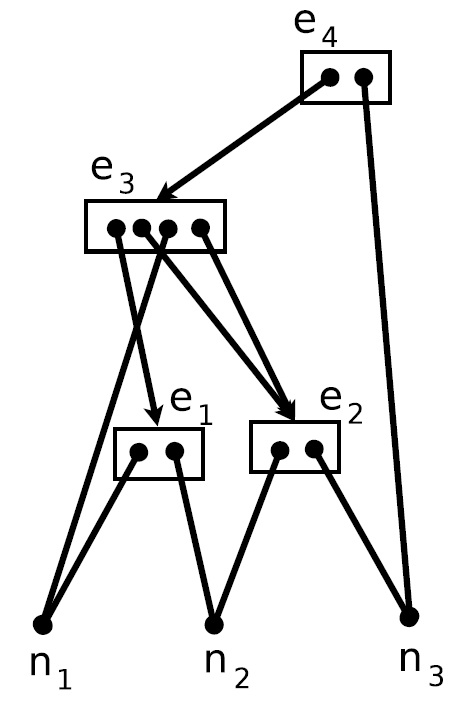
\includegraphics[width=0.4
\textwidth]{figures/Magistrale/metagraph_graph}
\caption[]{An example of a DAG.
\label{fig:metagraph_graph}}
\end{figure}

But in Metagraph, links are ordered lists, represented as boxes. Thus, to convert it in a DAG it is possible to collapse the boxes to single points or to dissolve the boxes entirely and replace a single arrow, from point-to-box, by many arrows, from point to each of the box elements.  \\
Whereas the node table is the same as the vertex table for the hypergraph, nevertheless the link table now requires both an outgoing-atom list and an incoming-link set.
Figure \ref{fig:metagraph_table} shows the result.

\begin{figure}
\centering
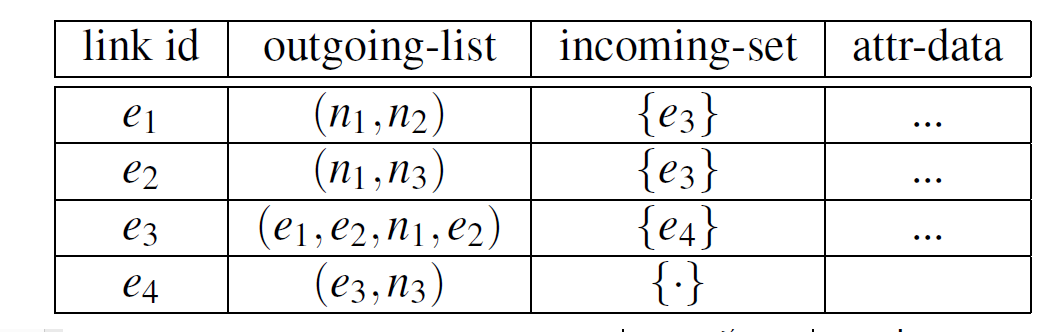
\includegraphics[width=0.8
\textwidth]{figures/Magistrale/metagraph_table}
\caption[]{Metagraph link table
\label{fig:metagraph_table}}
\end{figure}

For convenience, the name \enquote{Atom} is given to something that is either a node or a link. Links are then, sets of atoms. \\
These concepts are described in \cite{Vep20a, metagraph_app}, where RAM-usage considerations, reasons why metagraphs offer more efficient, more flexible and more powerful ways of representing graphs and reasons why a metagraph store is better than a graph store and much more, can also be found. \\

Finally, some extensions of the metagraph are considered: Typed Metagraph (TMG) and Directed Typed Metagraph (DTMG). \\
Typed metagraphs are defined as hypergraphs with types assigned to hyperedges and their targets, and the potential to have targets of hyperedges connect to whole links, as well as targets. 
An example can be found in Figure \ref{fig:typed_edge}. \\
A natural extension of a TMG is the Probabilistically TMG, based on probabilistic dependent types. Thus, one can assign a probability (or an entire probability distribution) to each connection between edges, thanks to the probabilistic type inheritance relations. In this way, it is possible to obtain a KB that can work with probabilistic logic, fuzzy logic, make uncertain inferences and much more. \\
Atomic Directed Typed Metagraphs (atomic DTMG) are introduced via partitioning the targets of each edge in a typed metagraph into input, output and lateral sets; one can then look at \enquote{metapaths} in which edges' output-sets are linked to other edges' input-sets (Figure \ref{fig:typed_metapath}). Thus, a DTMG is generally defined as a TMG composed by connecting DTMGs via metapaths, a recursive definition that bottoms out on the definition of atomic DTMGs. \\
For the whole theoretical formalism concerning TMG and DTMG refer to \cite{DBLP:journals/corr/abs-2012-01759}. 
That paper concludes by also describing useful types of morphisms that can be defined on a DTMG (catamorphisms, anamorphisms, histomorphisms, futumorphisms, hylomorphisms, chrono\-morphisms, metamorphisms and metachronomorphisms). 
They allow to formulate a wide variety of operations on metagraphs, which will not be described here. \\
The important thing to keep in mind is that the KB is used for AGI, so there will be many metagraphs and very large ones. Morphisms allow you to obtain simple and complex results by mutating/transforming/stretching/compressing the metagraph quickly and cleanly. \\

\begin{figure}
\centering
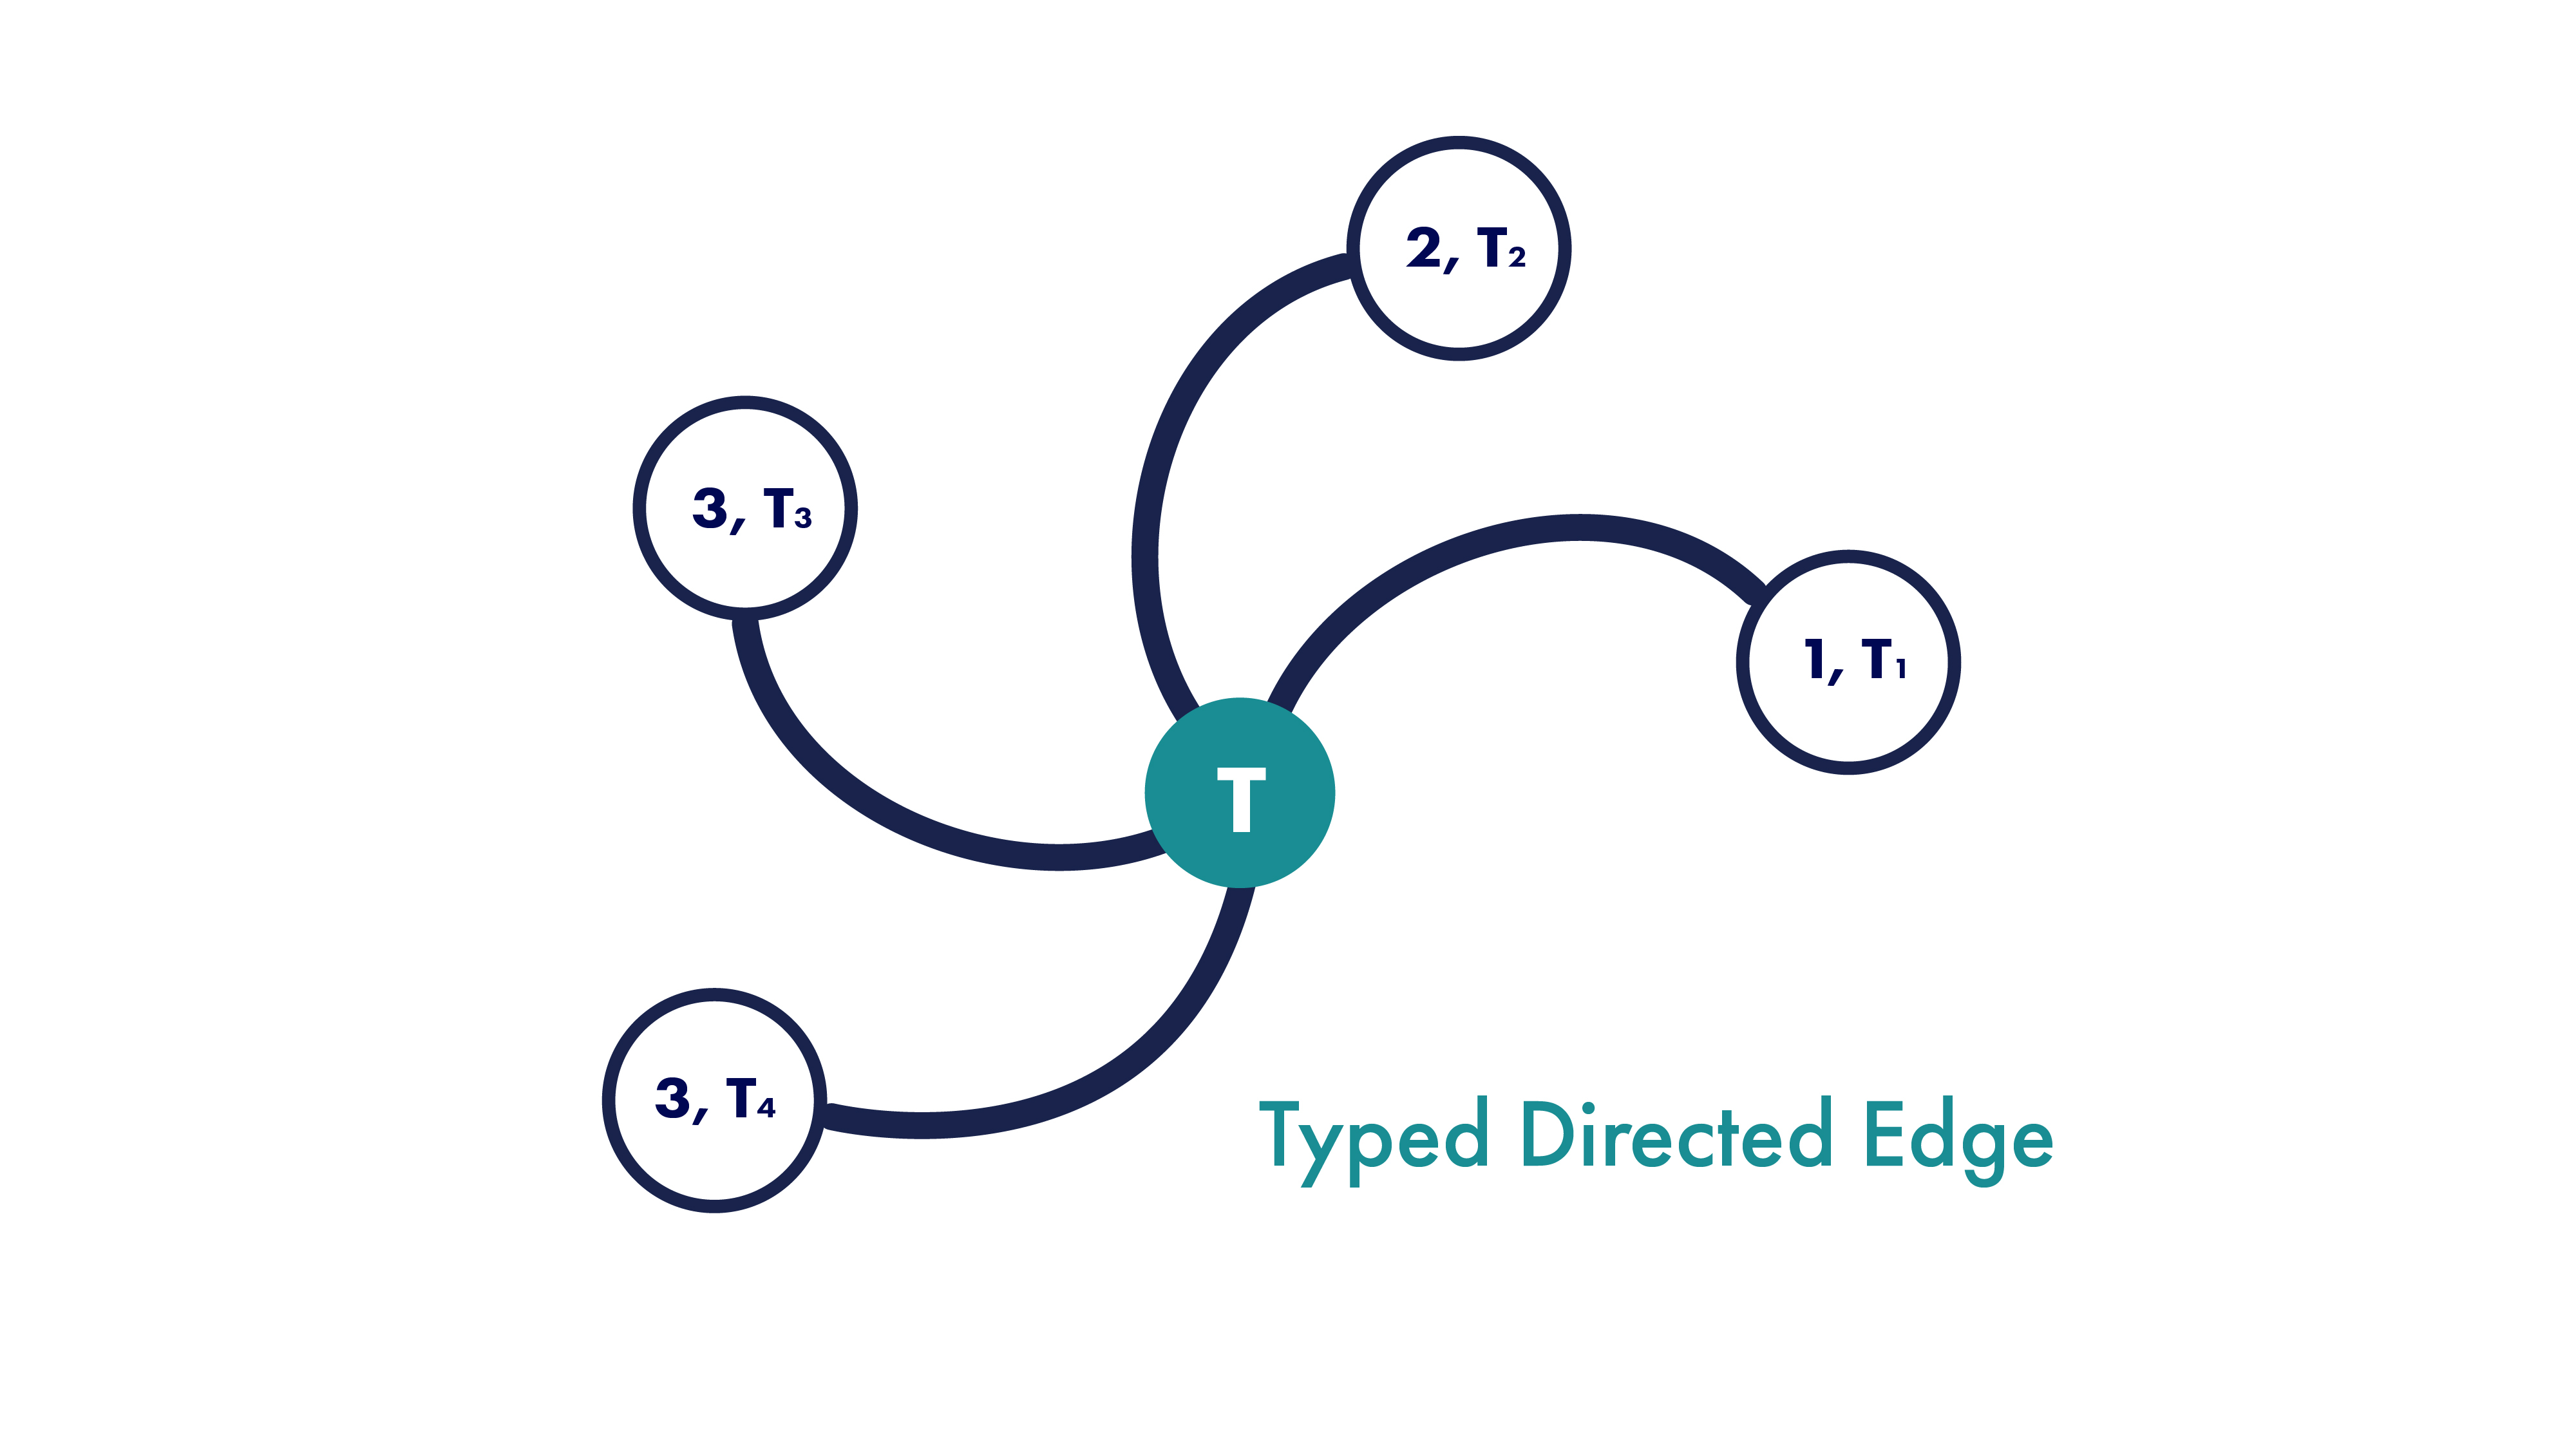
\includegraphics[width=0.6
\textwidth]{figures/Magistrale/typed_edge}
\caption[]{Example of a typed, directed edge. This one has 4 targets. $T$ is the type of the edge itself. The third and fourth targets are unordered relative to each other.
\label{fig:typed_edge}}
\end{figure}

\begin{figure}
\centering
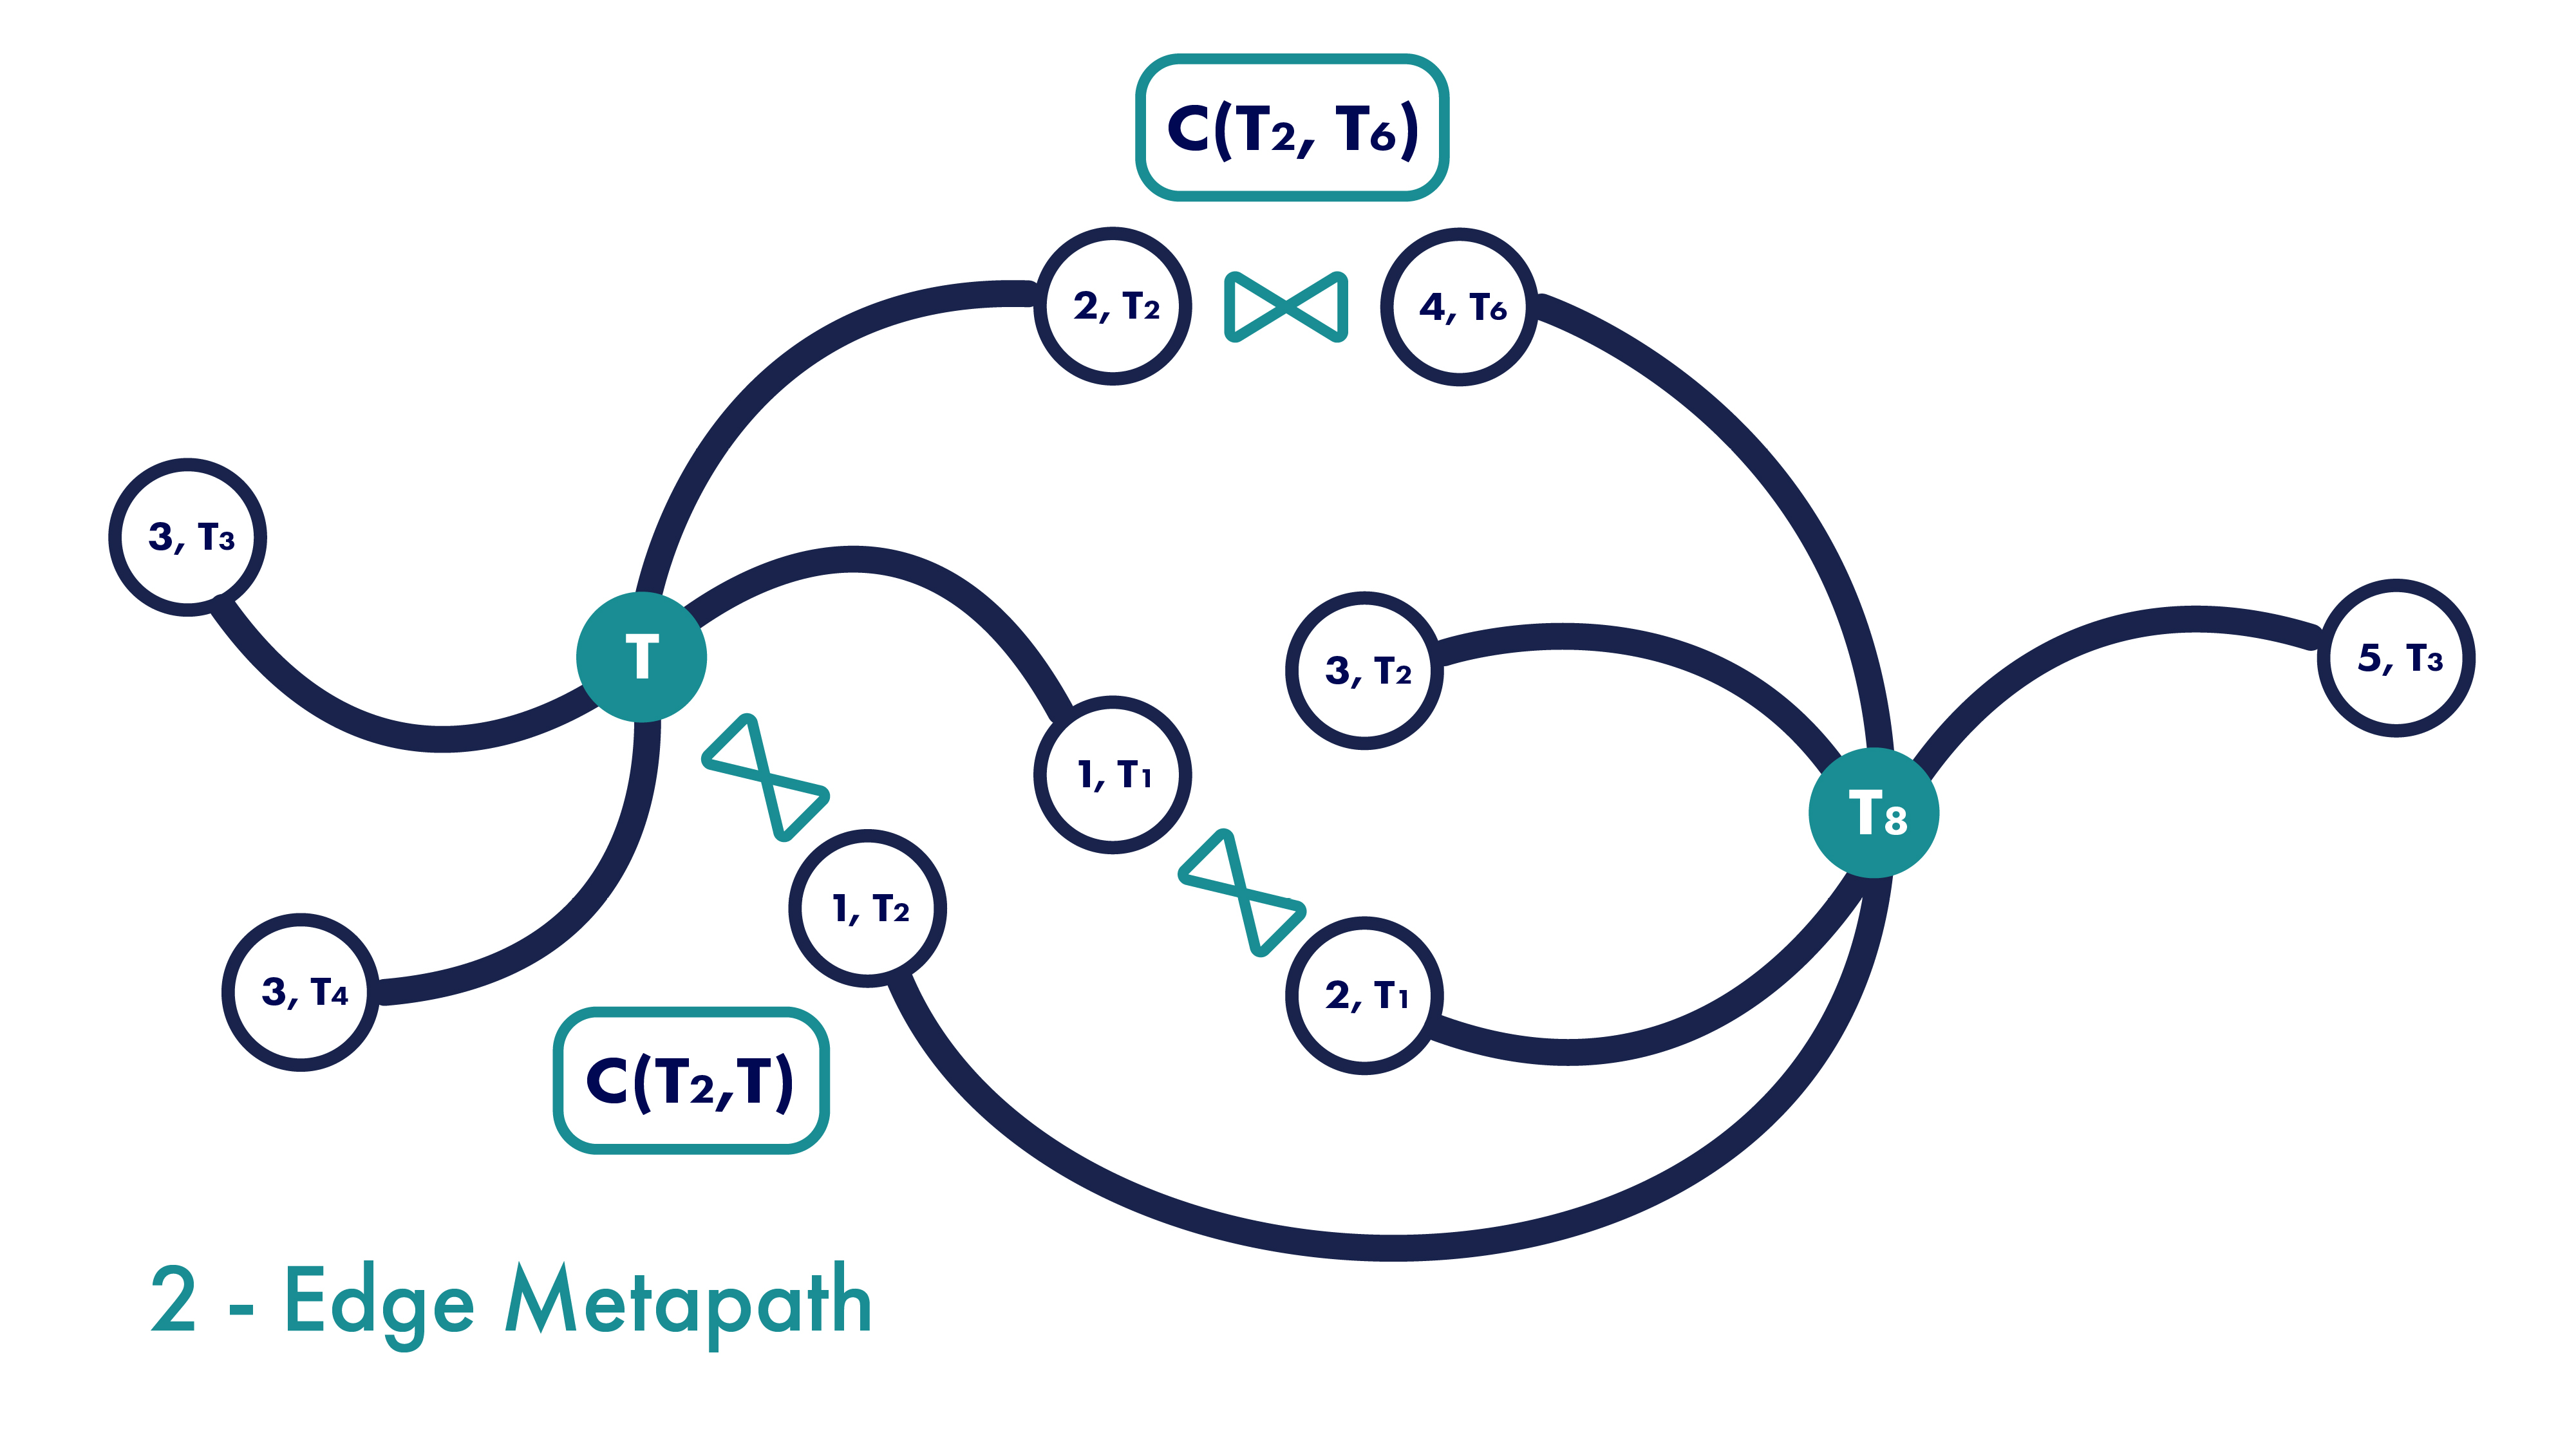
\includegraphics[width=0.65
\textwidth]{figures/Magistrale/typed_metapath}
\caption[]{A short metapath, formed by connecting two directed edges.
\label{fig:typed_metapath}}
\end{figure}

Last but not least, it is also useful to associate metagraph edges $E_i$ with nite lists $V_i$ of Values, each of which may be integer, floating-point or more complex in structure. The reason for these Values will be mentioned later.

\subsubsection{Atoms}\label{sec:atoms}

The vertices (nodes) and edges (links) of a graph (metagraph), known as Atoms, are used to represent not only \enquote{data}, but also \enquote{procedures} and then, many metagraphs are executable programs as well as data structures. \\
Atoms are one of the main components of the AtomSpace. Atoms, together with Values are what the AtomSpace stores.  \\
The two primary types of Atoms are Nodes and Links. They are used to represent anything that resembles a graph-theoretical graph. \\
From the TMG definition above, Atoms are typed (in the sense of Type Theory) and thus, they can be used to store a large variety of information. 
Values are used to assign \enquote{valuations} to Atoms, to indicate the truth or likelihood of that Atom, or to hold other kinds of transient data. Every Atom has a key-value database attached to it, that can store any kind of information about that Atom. The distinction between the \enquote{shape of the graph}, and its related \enquote{data} is central for allowing high-speed graph traversal and generalized graph query. Note that, in Ruby and Prolog programming languages, symbols are literally called atoms. Moreover, both LISP and Guile, allow parameters to be attached to symbols, as Values can be attached to Atoms. \\

When atoms are placed in the AtomSpace, they become unique. Thus, in comparison to other programming languages \footnote{Section \ref{sec:atomese} to understand why it is possible to talk about programming languages}, Atoms can be understood to be the same thing as symbols. The AtomSpace is essentially a symbol table, which commonly has the unique-symbols property.
Once an Atom is placed in the AtomSpace, it gets a single, unique ID. This unique ID is the string name of a Node and the outgoing set of a Link. \\
A TruthValue gives each Atom a valuation or an interpretation and conseguently, all Atoms in a given, fixed AtomSpace always carry a default valuation/interpretation along with them. Naturally, additional interpretations can be created. \\

The types form a type hierarchy: all atoms inherit from the type "Atom", and the type Atom itself inherits from ProtoAtom. The ProtoAtom is itself the base type for Values as well as Atoms. \\






\subsection{Pattern Engine and Unified Rule Engine}\label{sec:pattern_ur_engine}
\subsection{Atomese}\label{sec:atomese}
\subsection{Reasons}\label{sec:reasons}
% Distributed Atom Space - Architecture
% Atomspace come metagrafo
